\chapter{Canonical PCI-DSS Enterprise Scenarios}
\label{app:pci_scenarios}

This appendix provides the formal architectural and operational documentation for the canonical Payment Card Industry Data Security Standard (PCI-DSS) network scenarios utilized in the empirical baseline experiment by Allodi et al.~\cite{santos2017estimating} and incorporated into the HelpUS evaluation benchmark. The scenarios are derived directly from the authoritative PCI compliance treatise by Williams and Chuvakin~\cite{williams2014pci}.

\section{Scenario 1: Joe's Jumping Jerky Joint (Merchant Level 3)}
\label{sec:app_joe_scenario}
\subsection{Organizational Context and Compliance Scope}
Joe's Jumping Jerky Joint represents a small distributed merchant operating four brick-and-mortar storefronts alongside an e-commerce website accepting credit card payments. The business was notified by its payment acquirer that it qualifies as a Merchant Level 3 entity, mandating strict compliance validation with the PCI-DSS framework.

Each physical store utilizes IP-based Point-of-Sale (POS) terminals. In the baseline operational state (prior to compliance scoping), these POS terminals share physical and logical network infrastructure with non-payment systems:
\begin{itemize}
    \item Two store workstations used by managers to browse the web, handle email, and access order fulfillment portals.
    \item An unmanaged in-store marketing kiosk allowing customers to sign up for mailing lists.
    \item Unsegmented public Wi-Fi offered freely to customers visiting the store.
    \item An edge Digital Subscriber Line (DSL) business gateway equipped with DMZ functionality that was initially unconfigured.
\end{itemize}

\begin{figure}[htbp]
    \centering
    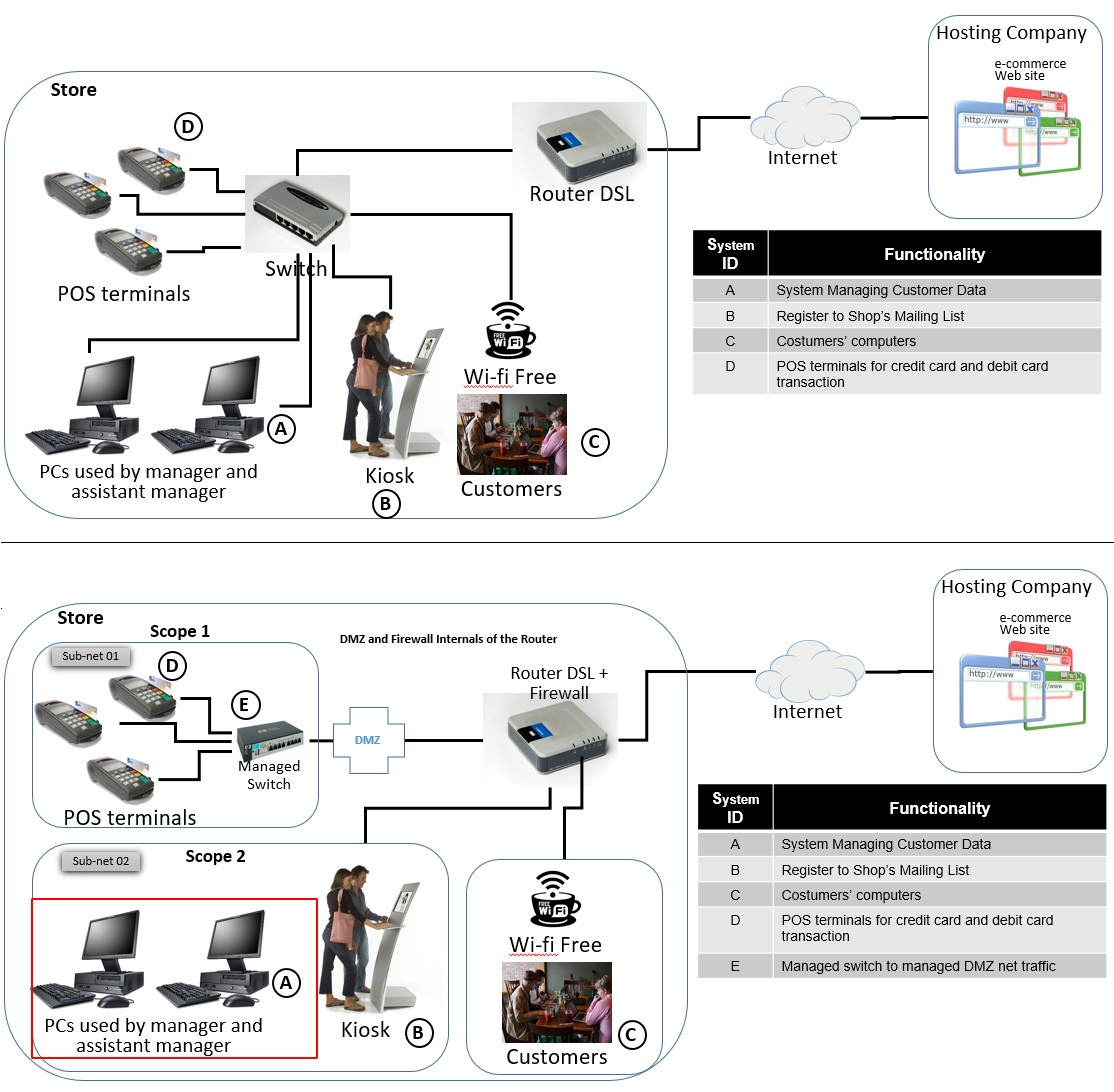
\includegraphics[width=0.92\linewidth]{figures/joebeforeandafter.jpg}
    \caption{Architecture of the Level 3 merchant network (Joe's Jumping Jerky Joint) before and after PCI-DSS network segmentation and DMZ enforcement~\cite{santos2017estimating, williams2014pci}.}
    \label{fig:app_joe_topology}
\end{figure}

\subsection{Architectural Remediation (After Compliance)}
To satisfy PCI-DSS scoping requirements (specifically Requirement 1 regarding firewall configurations and network segmentation), the merchant redeployed the infrastructure as shown in Figure~\ref{fig:app_joe_topology}:
\begin{enumerate}
    \item \textbf{Isolated POS DMZ Subnet:} The DMZ feature on the edge DSL router is activated. The IP-based POS devices are migrated to a dedicated, isolated physical subnet managed by an independent 8-port managed Ethernet switch.
    \item \textbf{Access Control and Ingress Filtering:} The DSL gateway firewall rules are locked down: no traffic originated from the administrative workstations, the kiosk, or the customer Wi-Fi is permitted to reach the POS devices or the POS controller.
    \item \textbf{Complete Wireless Isolation:} Guest Wi-Fi access is isolated into an independent logical broadcast domain with direct egress to the Internet, eliminating any local route to store management systems.
\end{enumerate}

\section{Scenario 2: Christine's Enterprise (Merchant Level 1)}
\label{sec:app_christine_scenario}
\subsection{Organizational Context and Core Switching Architecture}
Christine's company is a nationwide retail enterprise that expanded into a Merchant Level 1 organization. An internal security audit revealed that assessors had systematically underestimated the scope of PCI-DSS compliance because the corporate network was historically operated as a flat, unsegmented switching fabric.

Multiple legacy systems not involved in payment processing resided on the core corporate network. Because these legacy systems were no longer maintained by vendor software patches, they could not satisfy baseline PCI requirements. 

\begin{figure}[htbp]
    \centering
    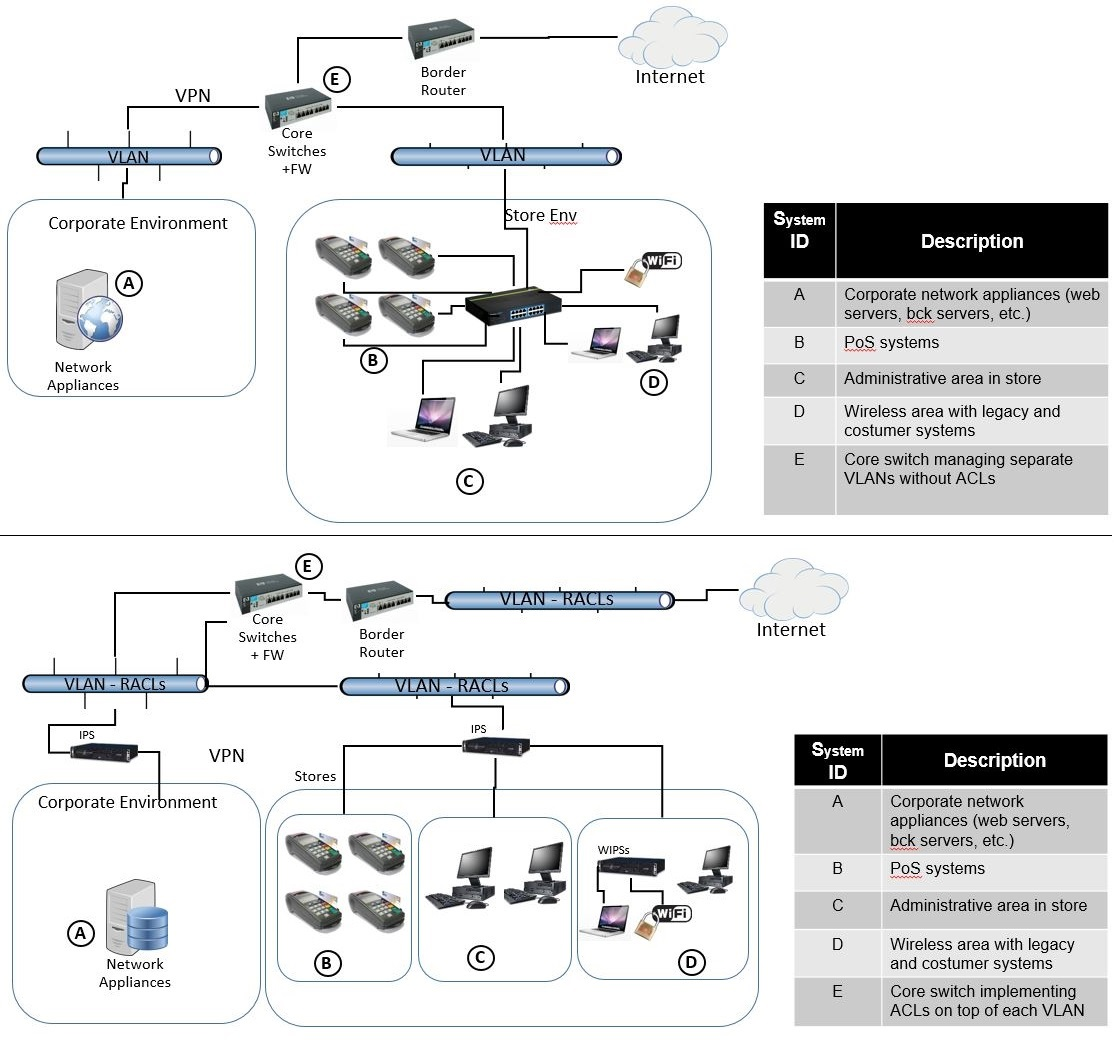
\includegraphics[width=0.95\linewidth]{figures/christinebeforeandafter.jpg}
    \caption{Architecture of the multi-tier enterprise network (Christine's Company) before and after core multi-VLAN segmentation and Router Access Control Lists (RACLs)~\cite{santos2017estimating, williams2014pci}.}
    \label{fig:app_christine_topology}
\end{figure}

\subsection{Multi-VLAN Remediation and RACL Enforcement}
To achieve compliance without undertaking a multi-million-dollar replacement of non-payment legacy systems, the enterprise deployed high-density aggregation switches (Cisco ASR series) equipped with hardware-enforced Router Access Control Lists (RACLs) and stateful firewall blades (Figure~\ref{fig:app_christine_topology}):
\begin{enumerate}
    \item \textbf{Cardholder Enclave Isolation:} The central payment processing servers and cardholder data repositories are isolated into dedicated VLANs protected by stateful inspection.
    \item \textbf{In-Store Point-of-Sale Segmentation:} Retail stores enforce RACLs that physically segregate POS terminals from administrative PCs and store kiosks.
    \item \textbf{Wireless Intrusion Prevention (WIPS):} Rogue access point detection and strict RACLs are activated across wireless access points to prevent air-interface bridging into the wired cardholder network.
    \item \textbf{Two-Factor VPN Bastion for Operators:} Technical administrators requiring access to cardholder systems are restricted to an Out-of-Band (OOB) management VRF protected by mandatory multi-factor authentication tokens.
\end{enumerate}
